\documentclass{article}
\usepackage{wrapfig}
\usepackage{float}
\usepackage{enumitem}
\usepackage{multirow}
\usepackage{longtable}
\usepackage{graphicx}
\usepackage{array}
\usepackage{amsmath}\usepackage{hyperref}
\graphicspath{ {report figures/} }
\usepackage{titlesec}
\usepackage[margin=1.5in]{geometry}
\geometry{a4paper, top=30mm, bottom=30mm}
\titleformat*{\section}{\large\bfseries}
\setlength{\skip\footins}{1cm}
\date{}
\author{He Ma u5893274}
\setlength{\parindent}{0pt}
\begin{document}
\title{\vspace{-1cm}System Engineering Assignment 2}
\maketitle
\section{Executive Summary}
Smart speakers are speakers that recognize voices, respond to voice commands and perform various tasks, such as playing music, providing information (like weather forecasts or news updates), controlling smart home devices (such as lights, thermostats, and locks), setting reminders, making calls, sending messages, and more. Most of smart speakers adopt artificial intelligence technology to process the voice command and wireless communication technologies to connect to smart phones or Ethernet, but other technologies will also be studied in this report.\\\\
In addition to the functions above, this report will propose a smart speaker that attempt to process command from users locally. If the attempt failed, it can utilize an external natural language processing server to process the voice command. Another key feature of the proposed design is that the signal filtering and interpretation of users' commands are performed in the same subsystem, which greatly reduces the overall complexity of the circuit.\\\\
\section{Functional Baseline}
In this section, the concept smart speaker will be reverse engineered into a functional baseline document. The functional baseline will not include the external voice processing server, instead it will only focus on the physical speaker device. All functions of the smart speaker and their relationships are shown in the function flow bock diagram (FFBD) below, where italic text represents the flow between functions.
\begin{figure}[H]
\centering
    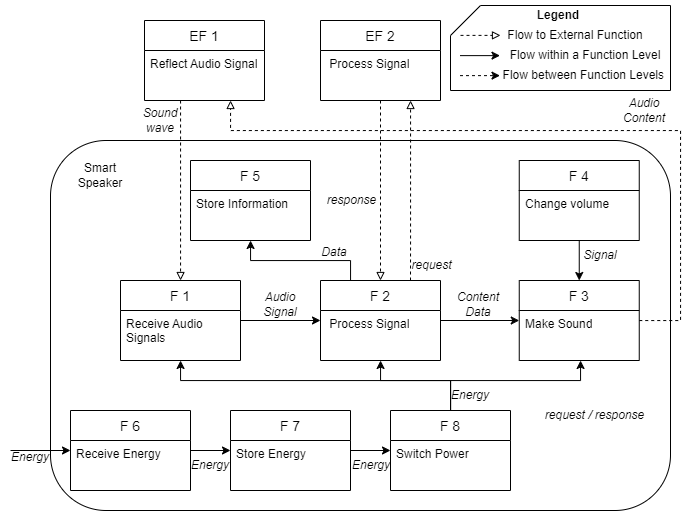
\includegraphics[scale=0.5]{FFBD1}
\end{figure}
The second level of FFBD is shown below where F2 and F3 are further decomposed. Note that power inputs are required to all the functions in second level FFBD but they are omitted to make the demonstration concise.
\begin{figure}[H]
\centering
    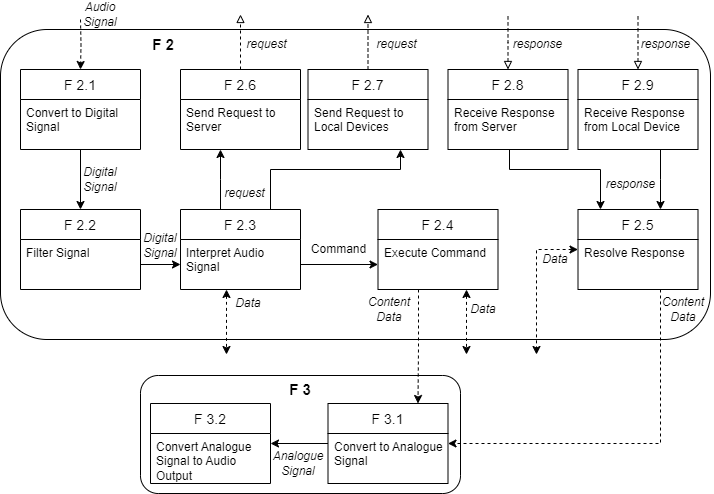
\includegraphics[scale=0.5]{FFBD2}
\end{figure}
All functions in the FFBD are reverse engineered from existing smart speakers on the market such as Google Home (Marteson 2020), Apple Homepod (Strong 2018) and Amazon Echo Dot  (Higgins 2016). Their descriptions are listed in the functional decomposition table below:
\begin{center}
\begin{longtable}{| m{.13\textwidth} | m{.17\textwidth} | m{.6\textwidth} |} 
 \hline
 Numbering & Functions & Description \\ 
 \hline\hline
 F 1 & Receive Audio Signals & Receive input audio signal which can be any sound including human voice and environmental.\\ 
 \hline
 F 2 & Process Signal & Decides the content to play according to the input audio signal. \\ 
 \hline
 F 3 & Make Sound & Play the content prepared in F 2 as audio output\\ 
 \hline
 F 4 & Change Volume & Change the output volume according to the input from users.\\ 
 \hline
 F 5 & Store Information & The speaker memorize previous audio input and output.\\ 
 \hline
 F 6 & Receive Energy & Input energy to the speaker and energy storage.\\ 
 \hline
 F 7 & Store Energy & Keep energy to sustain other functions that consume energy.\\ 
 \hline
 F 8 & Switch Power & Turn the speaker on and off.\\ 
 \hline
 F 9 & Indicate Power & Display the percentage of power left and whether the speaker is being charged.\\ 
 \hline
 
 F 2.1 & Convert to Digital Signal & convert the audio signal to digital electronic signal.\\ 
 \hline
 F 2.2 & Filter Signal & One function of filtering is to increase the signal to noise ratio. Another function is to split the signal to multiple channels. Different channels may represents audio input from various sources including the echo form the speaker itself, alternatively they can represent different frequency components in the signal.\\ 
 \hline
 F 2.3 & Interpret Audio Signal & Attempt to convert the input audio signal to a standardized command. If the interpreted command can be accomplished using local information, then request local processor to execute the command. Otherwise, if it is requesting resources from local devices, then send request to local devices. Otherwise, request external natural language processor to process the audio signal.\\ 
 \hline
 F 2.4 & Execute Command & If the command is simple and  well formatted, generate a content for output using local information.\\ 
 \hline
 F 2.5 & Resolve Response & Generate contents for output using the response from external information sources.\\ 
 \hline
 F 2.6 & Send Request to Server & Request external signal processor to generate contents for output.\\ 
 \hline
 F 2.7 & Send Request to Local Devices & Request local devices to provide output contents.\\ 
 \hline
 F 2.8 & Receive Response from Server & Receive the contents generated by external signal processor.\\ 
 \hline
 F 2.9 & Receive Response from Local Devices & Receive the contents provided by local devices. \\ 
 \hline
\end{longtable}
\end{center}
\section{Concept Selection}
One essential function of any smart speaker is how to interpret the voice command from users This function determines how smart the speaker is. Therefore, this function along with the Execute Command (F 2.4) and Filter Signal (F 2.2) functions will be studied further in this section. The signal filter not only remove noise, but also separate the user voice from the echo of the speaker itself. The Command Executor will fetch data from local memory as requested by the interpreted users' command. Together the 3 function blocks form a causal path that dominates key aspects of the design.\\\\
There are several options of technologies brainstormed to accomplish each of those 3 functions. The brainstorm utilize both my personal experience and the information searched online to ensure a wide variety of solutions are considered. Then several popular products on the market such as Google Home (Marteson 2020), Apple Homepod  (Strong 2018) and Amazon Echo Dot (Higgins 2016) are researched to explore potential combinations of their partial solutions to different problems. All possible ideas are documented in a table initially regardless their feasibility and drawbacks. At the end of brainstorming, solutions are considered against some benchmarks to select the best possible concept sketch. The benchmarks are listed in the table below:\\\\
\begin{center}
\begin{longtable}{| m{.17\textwidth} | m{.6\textwidth} | m{.13\textwidth} |} 
 \hline
 Name & Requirement & importance \\ 
 \hline\hline
 Supports & The smart speaker shall be updated regularly with newly developed voice recognition system available & 0.6\\ 
 \hline
 Adaptability & The smart speaker shall interpret the command differently in different context & 0.5\\ 
 \hline
 Cost & The cost to produce smart speaker shall be less than 500 dollar & 0.3\\ 
 \hline
 Response Time & The smart speaker shall take action or make response in less than 10 seconds & 0.3\\ 
 \hline
\end{longtable}
\end{center}
The solutions from brainstorming are shown in the concept combination table below. The combination of their numbering are used to represent concept sketches in the evaluation matrix later.\\
\begin{center}
\begin{longtable}{| m{.28\textwidth} | m{.3\textwidth} | m{.3\textwidth} |} 
 \hline
 F 2.2 Filter signal & F 2.3 Interpret Audio Signal & F 2.4 Execute Command \\ 
 \hline\hline
 Sol 1.1 Analogue filter & Sol 2.1 Dynamic time warping & Sol 3.1 Microprocessor \\ 
 \hline
 Sol 1.2 Digital fast Fourier transform & Sol 2.2 Hidden Markov models & Sol 3.2 Field Programmable Gate Arrays (FPGA) \\ 
 \hline
 Sol 1.3 Artificial neural networks & Sol 2.3 Artificial neural networks & Sol 3.3 central processing unit (CPU) \\ 
 \hline
\end{longtable}
\end{center}
A evaluation matrix shown below is used to compare different combinations of solutions above. The score of each solution against individual requirements are classified into 5 levels. A score of 0 means failing to meet the requirement. 1 means failing to the requirement but can be amended. 2 means barely meeting the requirements. 3 means meeting the requirement easily. 4 Means exceeding the requirement. The weighted sum of all scores are used to rank concept combinations.\\
\begin{center}
\begin{longtable}{| m{.23\textwidth} | m{.1\textwidth} | m{.15\textwidth} | m{.05\textwidth} | m{.14\textwidth} | m{.14\textwidth} |} 
 \hline
  Design Specification & Supports & Adaptability & Cost & Response Time & Weighted Sum \\ 
 \hline
  Sol 1.3 - 2.3 - 3.1 & 5 & 5 & 5 & 3 & 7.9\\ 
 \hline
  Sol 1.3 - 2.3 - 3.3 & 5 & 5 & 0 & 4 & 6.7\\ 
  \hline
  Sol 1.1 - 2.3 - 3.3 & 4 & 4 & 3 & 4 & 6.5\\   
 \hline
  Sol 1.3 - 2.1 - 3.1 & 3 & 2 & 4 & 5 & 5.5\\   
 \hline
  Sol 1.3 - 2.1 - 3.3 & 1 & 2 & 3 & 5 & 4\\   
 \hline
\end{longtable}
\end{center}

The combination with highest score in the evaluation matrix is using microprocessor to execute commands and using artificial neural network for both filtering signal and interpreting audio signal. Despite the cost of artificial neural network is bit higher than other technologies, using the same hardware to accomplish different functions can reduce the cost significantly. Thus a sketch of this selected concept design is shown below:\\
\begin{wrapfigure}{r}{.5\textwidth}
\centering
    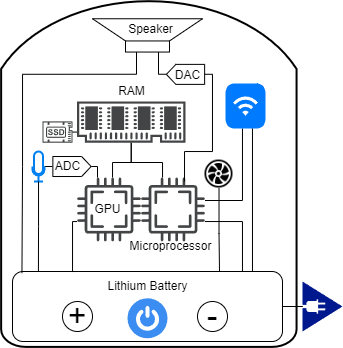
\includegraphics[scale=0.5]{Concept Sketch}
\end{wrapfigure}
The microphone is a dynamic microphone integrated with an analogue-digital converter (ADC). The Input signal is filtered and split into several channels using an artificial neural network program. The artificial neural network is implemented by the graphic processing unit. The connection to local devices and Ethernet is using Wi-Fi. The controlling electronic chip is a microprocessor. The volume switches and power switch are touch buttons. The hard drive is an Solid State Drives (SSD). The random access memory (RAM) is of Double Data Rate 5 (ddr5) type. The charger is a type-C charger. The speaker is a diaphragm speaker integrated with a digital-analogue converter (DAC).
\section{System Architecture}
Based on the optimal concept sketch selected in previous section, a physical system architecture can be designed as the diagram shown below, where italic text represents the flow between subsystems:\\
\begin{figure}[H]
\centering
    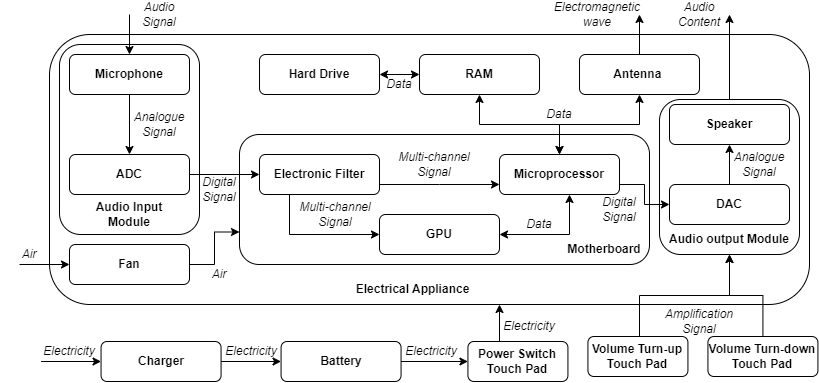
\includegraphics[scale=0.46]{Architecture}
\end{figure}
All the systems/subsystems shown in the diagram above are described in detail in the table below. The justifications of how subsystems and their interfaces are designed is are also included in the description of each subsystem:
\newlist{myitems}{enumerate}{3}
\setlist[myitems, 1]
{label=S\arabic{myitemsi}}
\setlist[myitems, 2]
{label=S\arabic{myitemsi}.\arabic{myitemsii}}
\setlist[myitems, 3]
{label=S\arabic{myitemsi}.\arabic{myitemsii}.\arabic{myitemsiii}}
\begin{myitems}
  \item \textbf{Electrical Appliance}: This subsystem groups all the components that consume electricity. This is because they need a common ground potential provided by the battery and thus a common power supply bus. In addition, they should be enclosed by a whole insulated frame. Such integrated architecture can greatly improve the overall performance of the system (Fathi 2015).
  \begin{myitems}
  	\item \textbf{Audio Input Module}: This subsystem convert the audio signal to digital data that can be processed by the subsequent subsystem. The speaker and the ADC are designed as an integrated structure because using commercial off-the-shelf (COTS) is cheaper and saves development time (Health, Sinclair \& Britain. 1995) and most of the COTS microphones on the market have integrated ADC within.
  	  \begin{myitems}
  	  \item \textbf{Microphone}
  	  \item \textbf{ADC}: Analogue-digital converter.
  	  \end{myitems}
  	\item \textbf{Motherboard}: This subsystem is where input audio is signal is processed and where output content is generated. Because signal processing and computation is an electronic current intensive task and they generate a lot of heat. Those electronic components needs to be placed together on a heat conducting frame and the frame needs to be placed in front of the fan.
  	\begin{myitems}
  	  \item \textbf{Electronic Filter}
  	  \item \textbf{Microprocessor}: This microprocessor needs to perform tasks exclusive for this smart speaker system such as deciding the data flow direction based on the data structure that is exclusive for the smart speaker. To meet this performance requirement, the microprocessor needs to be a customized integrated circuit.
  	  \item \textbf{GPU}: Despite there is no graphic processing function in the system, GPU is designed into the smart speaker because it adopts artificial neural network technology which performs best on GPU. GPU can also take the function of filtering signals which reduce the circuit complexity of the entire system. Lower complexity usually leads to cheaper production cost and more robust performance (Madhav Shridhar Phadke 1989).
  	  \end{myitems}
  	\item \textbf{Audio Output Module}: For the same reason as the Audio input module (Fathi 2015), the speaker and the DAC are integrated as one subsystem to improve the performance of the whole system.
  	\begin{myitems}
  		\item \textbf{DAC}: Digital-analogue converter.
  		\item \textbf{Speaker}
  	\end{myitems}
  	\item \textbf{Antenna}: Used to connect to Wi-Fi.
  	\item \textbf{RAM:} Random access memory chip.
  	\item \textbf{Hard Drive}: Solid State Drive is used for its small size and fast reading/writing speed.
  \end{myitems}
  \item \textbf{Charger}: The charger is a separate physical structure connected to smart speaker via a type-c USB cable.
  \item \textbf{Battery}: Lithium rechargeable battery is used.
  \item \textbf{Power Switch Touch Pad}
  \item \textbf{Volume Turn-up Touch Pad}
  \item \textbf{Volume Turn-down Touch Pad}
\end{myitems}
The corresponding functions in section 2 are allocated to each of the physical subsystems in the table below:
\begin{center}
\begin{tabular}{| m{.5\textwidth} | m{.5\textwidth} |} 
 \hline
  Functions & Subsystems \\ 
 \hline\hline
  F1 Receive Audio Signal & S1.1.1 Microphone \\   
 \hline
	F2  Process Signal & S1.2 Motherboard \\   
 \hline
  F2.1 Convert to Digital Signal & S1.1.2 ADC \\   
 \hline
 F2.2 Filter signal & \multirow{2}{*}{S1.2.3 GPU}\\
\cline{1-1}
 F2.3 Interpret Audio Signal &\\
\hline
	F2.4 Execute Command & \multirow{2}{*}{S1.2.2 Microprocessor}\\
\cline{1-1}
 F2.5 Resolve Response &\\
 \hline
	F2.6 Send Request to Server & \multirow{4}{*}{S1.5 Antenna}\\
\cline{1-1}
	F2.7 Send Request to Local Devices &\\  
\cline{1-1}
	F2.8 Receive response from Server &\\
\cline{1-1}
	F2.9 Receive Response from Local Device &\\
 \hline
  F3 Make Sound & S1.3 Audio Output Module \\
 \hline
 F3.1 Convert to Analogue Signal & S1.3.1 DAC \\
 \hline
 F3.2 Convert Analogue signal to Audio Output & S1.3.2 Speaker \\
 \hline
 	\multirow{2}{*}{F4 Change volume} & S5 Volume Turn-up Touch Pad\\
 	\cline{2-2} 
 	& S6 Volume Turn-down Touch Pad\\
 \hline
 \multirow{2}{*}{F5 Store Information} & S1.5 RAM\\
 	\cline{2-2} 
 	& S1.6 Hard Drive\\
 \hline
 F6 Receive Energy  & S2 Charger \\   
 \hline
 F7 Store Energy & S3 Battery \\   
 \hline
 F8 Switch Power & S4 Power Switch Touch Pad \\   
 \hline
\end{tabular}
\end{center}
\section{Recommendation}
By reverse engineer the functionality of a smart speaker and reassign technological realization for each function, a novel architecture is designed where the command from users can be firstly processed locally without communicating with external natural language processing server and only unsolvable commands needs to be passed to server. Hence, the processing time of the system can be greatly improved. The response time is one of the key aspect considered when comparing different concepts in section 3 and this recommended design scores relatively high comparing to other combinations of solutions.\\\\
Moreover, the signal filter and signal interpretation are both realized by artificial neural network to reduce the complexity of the circuit. In the concept comparison in section 3, the benefit of reduced complexity is reflected on the high score of cost when both Sol1.3 and Sol2.3 are adopted. Because artificial neural network performs massive parallel computations such as matrix multiplication, a GPU which is specialized in parallel computation (Tolga Soyata 2020) needs to be integrated to the motherboard.\\\\
Finally, this physical design architecture is verified against the functional baseline in section 2 and all functions are confirmed to be realized by corresponding subsystems of this recommended design.
\section*{Bibliography}
Madhav Shridhar Phadke 1989, \textit{Quality engineering using robust design}, Prentice Hall, Englewood Cliffs, N.J.\\\\
Fathi, M 2015, \textit{Integrated Systems: Innovations and Applications}, Springer.\\\\
Health, Sinclair, IJ \& Britain., G 1995, \textit{Use of Commercial Off-the-Shelf (Cots) Software in Safety-Related Applications}.\\\\
Strong, A 2018, \textit{What Is Apple Homepod}, Createspace Independent Publishing Platform.\\\\
Higgins, R 2016, \textit{Amazon Echo Dot}, Createspace Independent Publishing Platform.\\\\
Marteson, E 2020, \textit{Google Home: Learning the Basics}, Silver Starz.\\\\
Tolga Soyata 2020, \textit{Gpu Parallel Program Development Using Cuda}., Crc Press, S.L.
\end{document}